% figures/reality/target_vs_realized_geometry.tex
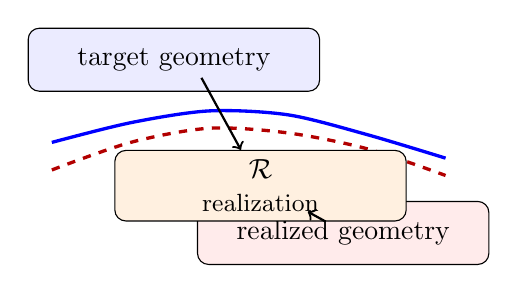
\begin{tikzpicture}[
  x=1cm,y=1cm,
  box/.style={draw, rounded corners, align=center, minimum width=3.7cm, minimum height=0.8cm},
  arrow/.style={->, thick}
]
\draw[very thick, blue] plot[smooth] coordinates {(0,0) (1,0.25) (2,0.4) (3,0.35) (4,0.1) (5,-0.2)};
\draw[very thick, red!70!black, dashed] plot[smooth] coordinates {(0,-0.35) (1,0.0) (2,0.18) (3,0.12) (4,-0.08) (5,-0.42)};

\node[box, fill=blue!8] at (1.55,1.05) {target geometry};
\node[box, fill=red!8] at (3.7,-1.15) {realized geometry};

\node[box, fill=orange!12] (R) at (2.65,-0.55) {$\mathcal R$\\\small realization};
\draw[arrow] (1.9,0.82) -- (R);
\draw[arrow] (R) -- (3.25,-0.88);
\end{tikzpicture}
